\documentclass{article}
\title{MEC 361 Assignment}
\author{Fidelugwuowo Dilibe. Reg No: 2018/248767}
\usepackage{graphicx}
\begin{document}
\maketitle
\newpage
\section*{Question 2.1}
An 80-m-long wire of 5-mm diameter is made of a steel with E = 200 GPa and an ultimate tensile strength of 400 MPa. If a factor of safety of 3.2 is desired, determine 
\begin{itemize}
\item the largest allowable tension in the wire
\item the corresponding elongation of the wire
\end{itemize}
\begin{center} \underline{Solution}\end{center}
%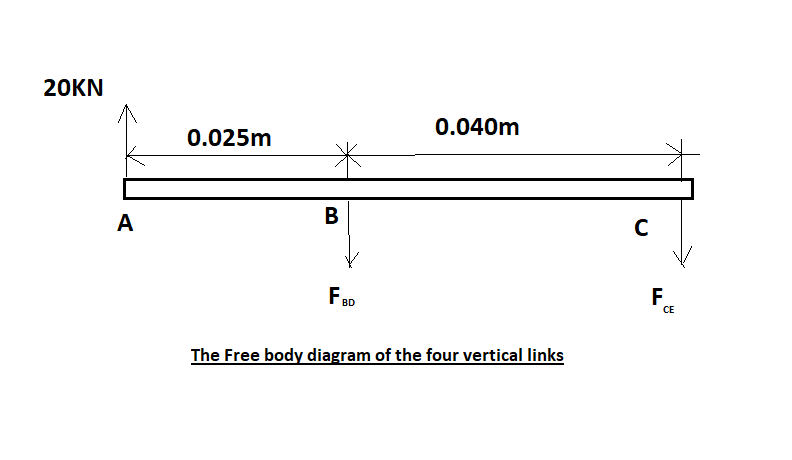
\includegraphics{1.7}
Given:\[L = 80m\]
\[E = 200GPa\]
\[d = 5mm\]
\[n=3.2\]
\[Formular: E = \frac{\sigma}{A}\]
\begin{center}Allowable stress, $ \sigma_{allow} = \frac{yield stress}{N}$\end{center}
\[\sigma_{alllow} = \frac{400 \times 10^{6}}{3.2} = 125MPa\]
 To find the extension,
\[e = \frac{\sigma}{E} = \frac{400 \times10^{6}}{200 \times 10^{9}} = 2 \times 10^{-3}\]
\begin{center} The value for the extension has no unit \end{center}
\section*{Question 2.9}
An aluminum control rod must stretch 0.08 in. when a 500-lb  tensile load is applied to it. Knowing that $\sigma_{ult} = 22ksi$ and $E = 10.1 \times 10^{6}psi$, determine the smallest diameter and shortest length that can be selected for the rod.
\begin{center} \underline{Solution}\end{center}
Given:
	\[\delta = 0.08in\]
	\[\sigma = 22 \times 10^{6}\]
	\[E = 10.1 \times 10^{6}psi\]
	\[P = 500lb\]
For the diameter:
\[A = \frac{\pi}{4}d^{2}\]
\[\sigma = \frac{P}{A}\]
Therefore \[A= \frac{P}{\sigma} = \frac{500}{22\times10^{6}} = 0.0227in^{2}\]
\begin{center} making d the subject of the formular, we get \end{center}
\[d = \sqrt{\frac{4\times2.27\times10^{-2}}{\pi} = 0.1701in}\]
For the shortest length, we have
\[E = \frac{\sigma}{e}, \space e = \frac{\delta}{L}\]
Therefore the equation above transcribe to
\[E = \frac{\sigma l}{\delta}\]
\begin{center} Making L the subject of the formular, \end{center}
\[l = \frac{E\delta}{\sigma}=\frac{10.1\times10^{6}\times0.08}{22\times10^{3}} = 36.72in\]


\section*{Question 2.15}
A 4-ft section of aluminum pipe of cross-sectional area 1.75$ in^{2}$ rests on a fixed support at A. The $\frac{5} {8}$-in.-diameter steel rod BC hangsfrom a rigid bar that rests on the top of the pipe at B. Knowing that the modulus of elasticity is $29 \times 10^{6}$ psi for steel and $10.4 \times 10^{6}$ psi for aluminum, determine the deflection of point C when a 15-kip force is applied at C.
\begin{center} \underline{Solution}\end{center}
Given:
\begin{center}Diameter of the Steel rod $d_{s}  = \frac{5}{8}in$ \end{center}
\begin{center}Length of the aluminium rod, $L_{A} = 4ft = 48in$ \end{center}
\begin{center}Length of the steel rod, $L_{S} = 7ft = 84in $\end{center}
\begin{center} Cross sectional Area of the alunimium, $A_{A} = 1.75in^{2}$\end{center}
\begin{center}Modulus of elasticity for aluminum, $E_{A} = 10.4 \times 10^{6}$ \end{center}
\begin{center}Modulus of elaticity for steel. $E_{S} = 29 \times 10^{6} $\end{center}
\begin{center}The force that $P = 15 \times 10^{3} $\end{center}
we will now find the cross cestional area of steel
\[A_{S} = \frac{\pi}{4}d_{S} = \frac{ \pi}{4} \times (\frac{5}{8})^{2} = 0.3068in^{2}\]
Deflection at c :
\[\delta_{c} = \delta_{A}+\delta_{S}\]
\[\delta_{A} = \frac{PL_{A}}{A_{A}E_{A}} = \frac{15 \times 10^{3} \times48}{1.75 \times 10.4 \times 10^{6}} = 0.03956in\]
\[\delta_{S} = \frac{PL_{S}}{A_{S}E_{S}} = \frac{15 \times 10^{3} \times84}{6.3068 \times 29 \times 10^{6}} = 0.14162in\]
\[\delta_{c} = \delta_{A}+\delta_{S}\]
\[\delta_{c} = 0.03956 + 0.14162 = 0.181in\]

\section*{Question 2.19}
Both portions of the rod ABC are made of an aluminum for which $E = 70 GPa$. Knowing that the magnitude of P is 4 kN, determine
\begin{enumerate}
\item  the value of Q so that the deflection at A is zero
\item  the corresponding deflection of B
\end{enumerate}
\begin{center}\underline{ Solution}\end{center}
Given: 
\[E = 70GPa = 70 \times 10^{9}Pa\]
\[P = 4KN = 4 \times 10^{3}N\]
\[d_{DB} = 20mm. \space \space d_{BC} = 6mm. \space \space d_{AB} = 0.4mm. \space \space d_{B2} = 0.5m. \space \space\]
Calculating the area of different parts of aluminum,
\[A_{AB} = \frac{\pi}{4}d^{2} = \frac{\pi}{4}{20\times 10^{-3}}^2 = 3.24  \times 10^{-4}m^{2}\]
\[A_{BC} = \frac{\pi}{4}d^{2} = \frac{\pi}{4}{60\times 10^{-3}}^2 = 2.827  \times 10^{-3}m^{2}\]
Using the method of superposition, we can assume that the forces acting at different points in the metal, sum up to zero.
\newline
Now for there to be zero deflection at A, 
\[\delta_{AB} = -\delta_{BC}\]
At section AB, 
\[\delta_{AB} = \frac{PL_{AB}}{A_{AB}E} = \frac{4\times 10^{3} \times 0.4}{3.14 \times 10^{-4} \times 70 \times 10^{9}}= 7.279\times10^{-6} \]
At section BC
\[\delta_{BC} = \frac{(P-Q)L_{BC}}{A_{BC}E} = \frac{(P-Q) \times 0.5}{2.827 \times 10^{-3} \times 70 \times 10^{9}}\]
\[=\frac{(P-Q)0.5}{2.125 \times 10^{-3}} = {(P-Q)2.52\times10^{-9}}\]
Following the statement we made for a zero deflection at A,
\[7.275\times10^{-5} =- (P-Q)2.52\times10^{-9}\]
\[7.275\times10^{-5} = -(1.010\times10^{-5})+ Q(2.52\times10^{-9})\]
\[8.285\times10^{-5} = (Q)2.52\times10^{-9}\]
\[Q = \frac{8.285\times10^{-5}}{2.52\times10^{-9}} = 32.97\times10^{3}N\]
For Deflection to occur at B,
\[\delta_{AB} = \delta_{B} = 7.275\times10^{-5}\]



\section*{Question 2.26}
The length of the $\frac{3}{32}in$.-diameter steel wire CD has been adjusted so that with no load applied, a gap of $\frac{1}{16}in$. exists between the end B of the rigid beam ACB and a contact point E. Knowing that$ E=29 \times 10^{6}$ psi, determinewhere a 50-lb block should be placed on the beam in order to cause contact between B and E.
\begin{center}\underline{ Solution}\end{center}
Given:
\begin{center}Length of string,$ L_{s} = 12.5 in$\end{center}
\begin{center}diameter of string,$d_{s} = \frac{3}{32}in$\end{center}
\begin{center}$E_{S} = 29 \times 10^{6}$\end{center}
\begin{center}$P = 50lb$\end{center}
Drawing a free body diagram of the syste, we have 
\newline
\includegraphics{untitled}
\newline
Taking moment about point A, we have
\[M_{A} = 4f_{s} - 50 (20 -x) = 0\]
but $f_{s} = ?$, However
\begin{center}$\delta_{s} = \frac{f_{s}L_{s}}{A_{s}E}$.  This implies that $f_{s} = \frac{\delta_{s}A_{s}E}{L_{s}}$\end{center}
\[\delta_{s} = 4 \theta\]
where 4 is th edistance fro the string to the point A
\newline
$\theta$ is the angle covered by the beam
\[\theta = \frac{\frac{1}{16}}{20} = 3.125 \times 10^{-3}rads\]
\[\delta_{s} = 4\times 3.235 \times 10^{-2} = 0.065in\]
\[A_{s} = \frac{\pi}{4} \times (\frac{3}{32})^{2} = 6.903 \times 10^{-3}in^{2}\]
\[F = \frac{0.0125 \times 6.903 \times 10^{-3} \times 29 \times 10^{6}}{12.5} = 200187lbs\]
Hence,
\[4f_{s} - 50(20-x) = 0\]
\[(4\times200.187) - 1000 + 50x = 0\]
\[800.748 - 1000 + 50x = 0\]
\[50x = 199252\]
\[ x = \frac{199.252}{50}\]
\[x = 3.985in\]



\section*{Question 2.35}
A 4-ft concrete post is reinforced with four steel bars, each with a $\frac{3}{4}in$ diameter. Knowing that $E_{s} = 29 \times 10^{6} psi$ and $E_{c}= 3.6 \times 10^{6} psi$, determine the normal stresses in the steel and in the concrete when a 150-kip axial centric force P is applied to the post.
\begin{center}\underline{ Solution}\end{center}
\begin{center}$ P = P_{c} + P_{s}$\end{center}
deformation of a steel bar and that of a concrete are equal, hence
\[\delta_{c} = \delta_{s}\]
\[\frac{P_{c}L_{c}}{A_{c}E_{c}} = \frac{P_{s}L_{s}}{A_{s}E_{s}}\]
making $P_{c}$ the subject of the formular, we have
\[P_{c} = \frac{P_{s}A_{c}E_{c}}{A_{s}E_{s}}\]
\[A_{s} = 4\times\frac{\pi}{4} \times(\frac{3}{4})^{2} = 1.767in^{2}\]
\[A_{s} = 8_{2} - A_{s}= 64 - 1.767 = 62.233in^{2}\]
Since $P_{c} = \frac{P_{s}A_{c}E_{c}}{A_{s}E_{s}}$
\[P = P_{c} + P_{s}\]
\begin{center} becomes\end{center}
\[P = \frac{P_{s}A_{c}E_{c}}{A_{s}E_{s}} + P_{s}\]
This then becomes
\[P = P_{s}\frac{A_{c}E_{c}}{A_{s}E_{s}} + 1\]
\[P = 150Kips = 180 \times 10^{3}lbs\]
\[150\times10^{3} = P_{s}(\frac{62.233\times3.6\times10^{6}}{1.767\times29\times10^{6}} + 1)\]
\[150 \times 10^{3} = P_{s}(4.372 + 1)\]
\[P_{s} = \frac{150\times10^{3}}{5.372}\]
\[P_{s} = 27922.56lbs\]
Therefore $P_{c} = 50000 - 27922.56 = 122077.44$
Normal Stress:
\[\sigma_{c} = \frac{P_{c}}{A_{c}} = \frac{122077.434}{62.233} = 1961.619psi\]
\[\sigma_{s} = \frac{P_{s}}{A_{s}} = \frac{27922.56}{1767} = 15802.24psi\]



\section*{Question 2.41}
\begin{center} \underline{Solution}\end{center}
The total deformation of the bar is
\[\delta =\delta_{AD} + \delta{E} = 0\]
Where $\delta_{AD}$ is as a result of the forces 60KN and 40KN
and $\delta_{E}$ is as a result of the reaction at E
\[\delta_{AD} = \frac{P_{1}L_{1}}{A_{B}E_{B}} + \frac{P_{2}L_{2}}{A_{B}E_{B}} + \frac{P_{3}L_{3}}{A_{S}E_{S}} + \frac{P_{4}L_{4}}{A_{S}E_{S}} \]
%\includegraphics{}
\[P_{1} = 0, P_{2}=P_{3}=40KN= 40\times10^{3}, p_{4}=100\times10^{3}\]
\[A_{1} = A_{2} = \frac{\pi}{4}\times(30\times10^{-3})^{2}=7.069\times10^{-4}\]
\[A_{3} = A_{4} = \frac{\pi}{4}\times(40\times10^{-3})^{2}=1.257\times10^{-4}\]
\[l_{1} = l_{2} = 100mm = 0.1\]
\[l_{3} = 120mm = 0.12\]
\[l_{4} = 180mm = 0.18\]
\[E_{s} = 200\times 10^{9}, E_{b} = 205\times10^{-3}\]
\[\delta_{AD} = 0 + \frac{40\times0.1\times10^{3}}{7.069\times10^{-3}\times105\times10^{9}}+\frac{40\times10^{3}\times0.12}{1.259\times10^{-3}200\times10^{4}} + \frac{100\times10^{3}\times0.18}{1.257\times10^{-3}\times200\times10^{4}}\]
\[=(5.384\times10^{-5}) + (1.909\times10^{-5}) + (7.16\times10^{-5}) = 14.458\times10^{-5}m\]
%\includegraphics{}
\[\delta_{E} = \frac{R_{E}\times 0.2}{7.069\times10^{-3}\times105\times10^{9}}+\frac{R_{E}\times0.3}{1.259\times10^{-3}200\times10^{4}}\]
\[=(6.695\times10^{-9}R_{E}) + (1.193\times10^{-3}R_{E}) = 3.886\times10^{-9}R_{E}\]
\begin{center} Equating $\delta_{E}$ and $\delta_{AD}$\end{center}
\[\delta_{E}= \delta_{AD}\]
\[ 14.458\times10^{-5}=3.886\times10^{-9}R_{E}\]
\[R_{E} = \frac{14.458\times10^{-5}}{3.886\times10^{-9}} = 37186.21 = 37.19KN\]
For reaction at A, $R_{A}$ we have
\[R_{E}+R_{A} = (40\times10^{3})+(60\times10^{3})\]
\[R_{A} = (100\times10^{3})=37186.21\]
\[=62813.786N\]
Deflection at point C
\[\delta_{C} = \delta_{AB} + \delta_{BC}\]
\[\delta_{C} = \frac{R_{A}L_{4}}{A_{B}E_{B}} + \frac{P_{A}L_{3}}{A_{S}E_{S}}\]
\begin{center} Where $P = R_{A} - 60\times10^{-3}$\end{center}
\[\frac{62813.786 \times 0.18}{1.257\times 10^{-3}\times 200\times 10^{9}}+\frac{(62813.786-60000)\times 0.12}{1.259\times10^{-3}200\times10^{4}}\]
\[(4.497\times10^{-5})+(1.34\times10^{-6})=4.63\times10^{-5}m\]





\section*{Question 2.58}
\begin{center} \underline{Solution}\end{center}
Given \[\sigma = -11ksi = -11\times 10^{3}\]
\[T_{1} = 75^{o}F\]
\[Z_{b} = 14in, L_{AC} = 18in\]
\[A_{B} = 2.4in^{2}\]
\[E_{B} = 15\times10^{6}psi\]
\[\alpha_{B}=15\times10^{-6}F^{-1}\]
\[A_{AC} = 2.8in^{2}\]
\[E_{AC} = 10.6\times10^{6}psi\]
\[\alpha_{AC}=12.9\times10^{-6}F^{-1}\]
\begin{center}Pressure,$P = -\sigma_{AL}A_{AL}=- (11\times10^{3})(2.8) = -30800N$\end{center}
%\includegraphics{}
\[p_{1} = P_{2} = P\]
deformation as a result of force, P
\[F_{P} = \frac{P_{1}L_{B}}{A_{B}E_{B}} + \frac{P_{2}L_{AL}}{A_{AL}E_{AL}}\]
\[=\frac{-30800\times14}{2.4\times15\times10^{6}} + \frac{-30800\times18}{2.8\times10.6\times10^{6}}\]
\[=-0.012 - 0.0187 = -0.0307in\]
Deformation due to the thermal stress,
\[f_{T} = \delta_{P}+\delta = 0.0307 + 0.02 = 0.0507\]
\begin{center}But $F_{T} = \alpha_{B}\triangle T L_{B} +  \alpha_{AL}\triangle T L_{AL}$\end{center}
\[= \triangle T( \alpha_{B} L_{B} +  \alpha_{AL} L_{AL})\]
\[\triangle T(1.2\times 10^{-6}\times14 + 12.9\times10^{-6}\times18)\]
\[=\triangle T(4.002\times10^{-4})\]
\begin{center} Equating it$ \delta_{T} = 0.0507$, we have\end{center}
\[\triangle T(4.002\times20^{-4}) = 0.0507\]
\[\triangle T = \frac{0.0507}{4.002\times10^{-4}} = 126.69\]
$T_{2}$, new temperature for stress of $-11ksi$ to be experienced by aluminium = $\triangle T +T_{1}$
\[=126.69 + 75\]
\[T_{2} = 201.68^{o}F\]
\newline
\newline

\[F_{A} = L_{AL}\alpha_{AL}(\triangle T) - \frac{PL_{AL}}{E_{AL}A_{AL}}\]
\[=(18)(2.9\times10^{-6})(26.6) = \frac{30800\times 18}{10.6\times10^{6}\times2.8} = 10.712\times10^{-3}\]
\[L_{exact} = 18 + 10.712\times 10^{-3} = 18.0107in\]




\section*{Question 2.65}
\begin{center}\underline{ Solution}\end{center}
\[length, L = 2.5m\]
\[Outside\space diameter, d_{0} = 300mm = 0.3m\]
\[thickness, t =15mm = 0.015m\]
\[E = 200GPa = 200\times10^{9}Pa\]
\[v=0.30\]
\[P = 700KN = 700\times10^{3}N\]
\begin{itemize}
\item Change in length of the pipe,$\delta$
\[\delta  = \frac{-PL}{AE}\]
\[Area, A = \frac{\pi}{4}\times({{d_{0}}^{2}} - {{d_{1}}^{2}})\]
\[d_{1} = d_{0} - 2t = 0.3-2(0.15)=0.27\]
\[A = \frac{\pi}{4}(0.3^{2} - 0.27^{2}) = 0.0134m^{2}\]
\[\delta = \frac{(700\times10^{3})(2.5)}{(0.0134)(200\times10^{9})} = -6.53\times10^{-4}\]
\item Change in the outer diameter $\triangle d_{0}$
\[\triangle d_{0} = E_{lateral} \times d_{0}\]
but 
\[E_{lateral} = -\nu E_{axial}\]
\[E_{axial} = \frac{\delta}{L} = \frac{-6.53\times 10^{-4}}{2.5}=-2.612\times10^{-4}\]
\[E_{lateral} = -(0.30)(-2.612\times10^{-4}) = 7.836\times10^{-6}\]
\[\triangle d_{0} = 7.836\times10^{-5}\times0.3=2.3508\times10^{-5}m\]
\item Change in thickness, $\triangle t$
\[\triangle = E_{lateral} \times t_{0}= 7.836\times10^{-5}\times0.015=11.1754\times10^{-6}m\]

\end{itemize}





\section*{Question 2.81}
\begin{center} \underline{Solution}\end{center}
\[G = 12MPa = 12\times10^{6}\]
\[L - 100mm = 0.1m\]
\[P = 45KN = 45\times10^{3}N\]
\[a = ?, \space b=?\]
\[\tau = 1.4MPa = 1.4\times10^{6}\]
\[\delta = 5mm = 5\times10^{-3}m\]
%\includegraphics
\[F = \frac{1}{2}P = \frac{45\times10^{3}}{2} = 22.5\times10^{3}N\]
Finding b, bc = A but A= ? \[\tau = \frac{F}{A} \Rightarrow A= \frac{F}{\tau} = \frac{22.5\times10^{3}}{1.4\times10^{6}} = 0.0161m^{2}\]
\[bc=A \Rightarrow b= \frac{A}{C}=\frac{0.0161}{0.1} = 0.1607m\]
Finding a, \[r = \frac{\delta}{a} \Rightarrow a = \frac{\delta}{r}\]
\[r = \frac{\tau}{G} = \frac{1.4\times10^{6}}{12\times10^{6}}=0.1167\]
subsitituting into $a=\frac{\delta}{r}$
\[a = \frac{5\times10^{-3}}{0.1167} = 0.0428m\]

\end{document}